\documentclass{article}

% Symbols
\usepackage{amsfonts, amsthm}
\usepackage{upgreek}
\usepackage{physics}
\usepackage{cancel}
\usepackage{amssymb, latexsym, amsmath}
\usepackage{ stmaryrd }

%Algorithms
\usepackage[ruled,lined,linesnumbered,commentsnumbered]{algorithm2e}

%% Identación
\setlength{\parindent}{0cm}

% Comentario en bloques:
\iffalse
\fi

% Hipervínculos:
\usepackage{hyperref}

% Código
\newcommand{\code}[1]{\textcolor{white!25!black}{\texttt{#1}}}
\usepackage{listings}

%AMS
\usepackage{amsthm}
\newtheorem{algo-thm}{Algoritmo}

% Proof
\renewcommand*{\proofname}{\textbf{Soluci\'on:}}
% Theorem
\newtheorem*{theorem}{Teorema}

% Graphics
\usepackage{graphicx}
\usepackage{pgf}

% Color a letras.
%\usepackage[usenames,dvipsnames,svgnames,table]{xcolor}

% Tikz
\usepackage{tkz-graph}
\usepackage{tikz}
\usetikzlibrary{arrows,automata}
\usepackage{tikz}
\usetikzlibrary{arrows,automata}
%\usetikzlibrary[topaths]

% Def. Dr. César.
\usetikzlibrary{shapes,calc}
\tikzstyle{edge}=[shorten <=2pt, shorten >=2pt, >=stealth, line width=1.1pt]
\tikzstyle{edgeDotted}=[shorten <=2pt, shorten >=2pt, >=stealth, line width=1.1pt, dashed] %  dashed
\tikzstyle{edgeC}=[curve to, out=270,in=270,relative, dashed]
\tikzstyle{blueE}=[shorten <=2pt, shorten >=2pt, >=stealth, line width=1.5pt, blue]
\tikzstyle{redE}=[shorten <=2pt, shorten >=2pt, >=stealth, line width=1.5pt, red]
\tikzstyle{blackV}=[circle, fill=black, minimum size=6pt, inner sep=0pt, outer sep=0pt]
\tikzstyle{brownV}=[circle, fill=brown, draw, minimum size=6pt, line width=0.75pt, inner sep=0pt, outer sep=0pt]
\tikzstyle{blueV}=[circle, fill=blue, draw, minimum size=6pt, line width=0.75pt, inner sep=0pt, outer sep=0pt]
\tikzstyle{redV}=[circle, fill=red, draw, minimum size=6pt, line width=0.75pt, inner sep=0pt, outer sep=0pt]
\tikzstyle{redSV}=[semicircle, fill=red, minimum size=3pt, inner sep=0pt, outer sep=0pt, rotate=225]
\tikzstyle{blueSV}=[semicircle, fill=blue, minimum size=3pt, inner sep=0pt, outer sep=0pt, rotate=225]
\tikzstyle{blackSV}=[semicircle, fill=black, minimum size=3pt, inner sep=0pt, outer sep=0pt, rotate=225]
\tikzstyle{vertex}=[circle, draw, minimum size=6pt, line width=0.75pt, inner sep=0pt, outer sep=0pt]

% Margins
\addtolength{\voffset}{-1.5cm}
\addtolength{\hoffset}{-1.5cm}
\addtolength{\textwidth}{3cm}
\addtolength{\textheight}{3cm}

% Columnas multiples
\usepackage{multicol}

%Header-Footer
\usepackage{fancyhdr}
\renewcommand{\headrulewidth}{1pt}

\newcommand{\set}[1]{
  \left\{ #1 \right\}
}

%\pagenumbering{gobble} -- Este comando
%                       -- quita el número de página.
\footskip = 50pt
\renewcommand{\headrulewidth}{1pt}

\pagestyle{fancyplain}

\begin{document}
\title{UNIVERSIDAD NACIONAL AUT\'ONOMA DE M\'EXICO\\ Facultad de Ciencias}
\author{Autor: Adri\'an Aguilera Moreno}
\date{}
\maketitle
\begin{center}
  
\includegraphics[scale=0.20]{../Imagen/Portada.jpg}\\[0.4cm]
  \Large
  \bf{Geometría Computacional}
  \normalsize
\end{center}
\newpage
\fancyhead[r]{ Geometría Computacional.}
%%%%%%%%%%%%%%%%%%%%%%%%%%%%%%%%%%%%%%%%%%%%%%%%%%%%%
\section*{\LARGE{Tarea 01}}
\textbf{1.} Sea $S$ un conjunto de puntos en el plano en posición general. Demuestra que el
cierre convexo de $S$ es el polígono convexo con perímetro y área más pequeños que contienen a $S$.
\newline

\textbf{\textit{Dem.}} Para este problema, dividamos la prueba en dos posibles casos:
\begin{itemize}
\item Con $C(S)$\footnote{Diremos que $C$ es la función que nos devuelve como imagen el cierre convexo del conjunto de puntos
que se pase como argumento.} el cierre convexo. $C(S)$ es el polígono convexo con perímetro más pequeño que contiene a $S$.
  \newline
  Prueba por \textit{reducción al absurdo}. Supongamos que $C(S)$ no es el polígono de perímetro mínimo que envuelve
  todos los puntos en $S$. La suposición anterior implica que existe $C(S)' \not= C(S)$ tal que $P(C(S)') < P(C(S))$\footnote{Diremos
  que $P$ es la función que se mapea al perímitro del polígono que se pasa como argumento.} con $C(S)'$ un segundo cierre convexo. Entonces,
  ¿Cómo modificar $C(S)$ para convertirlo en $C(S)'$? Esto puede ocurrir en 3 casos, estos son:
  \newline
  
  \hspace*{0.5cm} \textit{Caso 1.} Existe un punto interno al polígono que lo convierte en uno de menor perímetro,
  en este caso perdemos convexidad en la nueva figura y por tanto debemos descartar este caso (pues esta condición es parte
  del antecedente de nuestra implicación).
  %%%%%%%%%%%%%%%%%%%%%%%%%%%%%%%%%%%%%%%%%%%%%%%%%%%%%%%%%%%%%%%%%%%%%%%%%% FIGURE 1
  \begin{figure}[ht!]
    \centering
    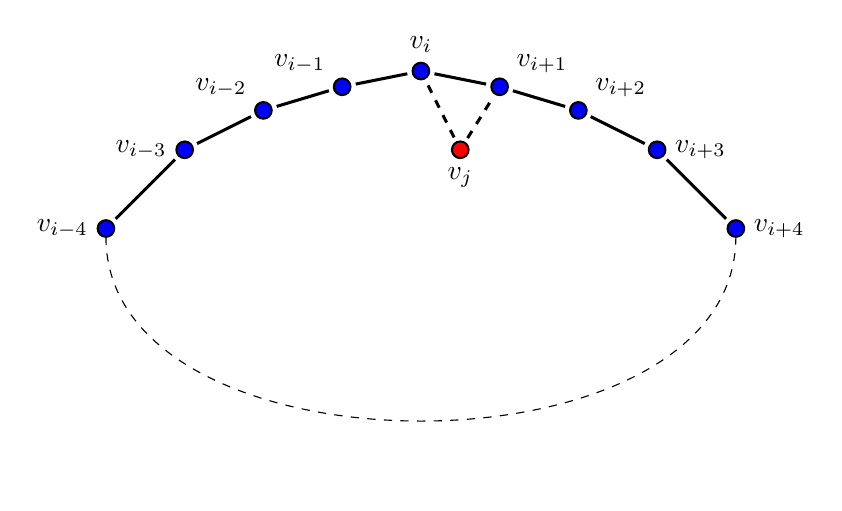
\begin{tikzpicture}
      \node(0) [blueV, label=180:$v_{i-4}$] at (-4, 3){};
      \node(1) [blueV, label=180:$v_{i-3}$] at (-3, 4){};
      \node(2) [blueV, label=150:$v_{i-2}$] at (-2, 4.5){};
      \node(3) [blueV, label=150:$v_{i-1}$] at (-1, 4.8){};
      \node(4) [blueV, label=90:$v_i$] at (0, 5){};
      \node(5) [blueV, label=0:$v_{i+4}$] at (4, 3){};
      \node(6) [blueV, label=0:$v_{i+3}$] at (3, 4){};
      \node(7) [blueV, label=30:$v_{i+2}$] at (2, 4.5){};
      \node(8) [blueV, label=30:$v_{i+1}$] at (1, 4.8){};
      \node(ext) [redV, label=270:$v_{j}$] at (0.5, 4){};
      \draw[edgeC] (0) to (5);
      \draw[edge] (0) to (1);
      \draw[edge] (1) to (2);
      \draw[edge] (2) to (3);
      \draw[edge] (3) to (4);
      \draw[edge] (4) to (8);
      \draw[edge] (5) to (6);
      \draw[edge] (6) to (7);
      \draw[edge] (7) to (8);
      \draw[edgeDotted] (ext) to (4);
      \draw[edgeDotted] (ext) to (8);
    \end{tikzpicture}
  \end{figure}
  %%%%%%%%%%%%%%%%%%%%%%%%%%%%%%%%%%%%%%%%%%%%%%%%%%%%%%%%%%%%%%%%%%%%%%%%%%
  
  \hspace*{0.5cm} \textit{Caso 2.} Existe un punto, extra en $C(S)'$ y que no esta en $C(S)$, sobre un segmento
  de $C(S)$, esto no reduce el perímetro y por tanto podemos descartar este caso.
  %%%%%%%%%%%%%%%%%%%%%%%%%%%%%%%%%%%%%%%%%%%%%%%%%%%%%%%%%%%%%%%%%%%%%%%%%% FIGURE 2
  \begin{figure}[ht!]
    \centering
    \begin{tikzpicture}
      \node(0) [blueV, label=180:$v_{i-4}$] at (-4, 3){};
      \node(1) [blueV, label=180:$v_{i-3}$] at (-3, 4){};
      \node(2) [blueV, label=150:$v_{i-2}$] at (-2, 4.5){};
      \node(3) [blueV, label=150:$v_{i-1}$] at (-1, 4.8){};
      \node(4) [blueV, label=90:$v_i$] at (0, 5){};
      \node(5) [blueV, label=0:$v_{i+4}$] at (4, 3){};
      \node(6) [blueV, label=0:$v_{i+3}$] at (3, 4){};
      \node(7) [blueV, label=30:$v_{i+2}$] at (2, 4.5){};
      \node(8) [blueV, label=30:$v_{i+1}$] at (1, 4.8){};
      \node(ext) [redV, label=270:$v_{j}$] at (0.5, 4.95){};
      \draw[edgeC] (0) to (5);
      \draw[edge] (0) to (1);
      \draw[edge] (1) to (2);
      \draw[edge] (2) to (3);
      \draw[edge] (3) to (4);
      %\draw[edge] (4) to (8);
      \draw[edge] (4) to (ext);
      \draw[edge] (ext) to (8);
      \draw[edge] (5) to (6);
      \draw[edge] (6) to (7);
      \draw[edge] (7) to (8);
    \end{tikzpicture}
  \end{figure}
  %%%%%%%%%%%%%%%%%%%%%%%%%%%%%%%%%%%%%%%%%%%%%%%%%%%%%%%%%%%%%%%%%%%%%%%%%%

  \hspace*{0.5cm} \textit{Caso 3.} Este caso lo anexo solo para estar completo,
  pero no debe suceder por la definición de $C(S)$, pues es el polígono convexo formado
  por la envolvente convexa del conjunto de puntos en $S$, así no debe haber un punto
  que no quede interno de $C(S)$ y en consecuencia de $C(S)'$.
  %%%%%%%%%%%%%%%%%%%%%%%%%%%%%%%%%%%%%%%%%%%%%%%%%%%%%%%%%%%%%%%%%%%%%%%%%% FIGURE 2
  \begin{figure}[ht!]
    \centering
    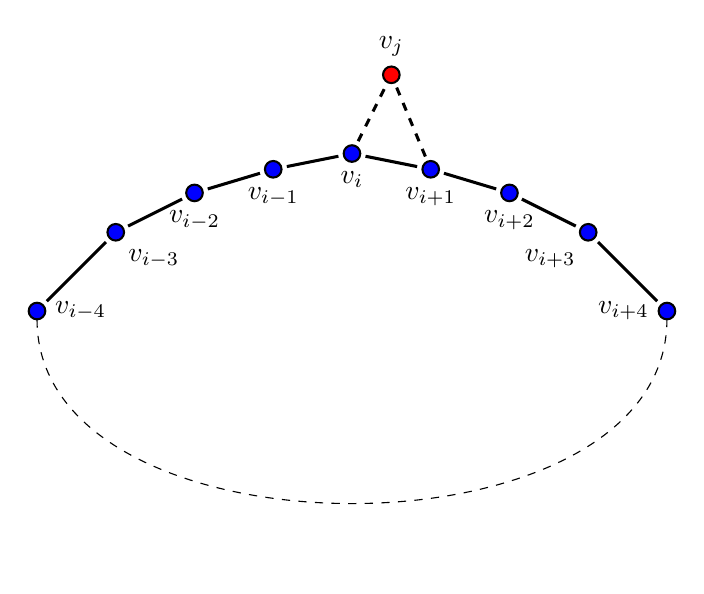
\begin{tikzpicture}
      \node(0) [blueV, label=0:$v_{i-4}$] at (-4, 3){};
      \node(1) [blueV, label=290:$v_{i-3}$] at (-3, 4){};
      \node(2) [blueV, label=270:$v_{i-2}$] at (-2, 4.5){};
      \node(3) [blueV, label=270:$v_{i-1}$] at (-1, 4.8){};
      \node(4) [blueV, label=270:$v_i$] at (0, 5){};
      \node(5) [blueV, label=180:$v_{i+4}$] at (4, 3){};
      \node(6) [blueV, label=250:$v_{i+3}$] at (3, 4){};
      \node(7) [blueV, label=270:$v_{i+2}$] at (2, 4.5){};
      \node(8) [blueV, label=270:$v_{i+1}$] at (1, 4.8){};
      \node(ext) [redV, label=90:$v_{j}$] at (0.5, 6){};
      \draw[edgeC] (0) to (5);
      \draw[edge] (0) to (1);
      \draw[edge] (1) to (2);
      \draw[edge] (2) to (3);
      \draw[edge] (3) to (4);
      \draw[edge] (4) to (8);
      \draw[edgeDotted] (4) to (ext);
      \draw[edgeDotted] (ext) to (8);
      \draw[edge] (5) to (6);
      \draw[edge] (6) to (7);
      \draw[edge] (7) to (8);
    \end{tikzpicture}
  \end{figure}
  %%%%%%%%%%%%%%%%%%%%%%%%%%%%%%%%%%%%%%%%%%%%%%%%%%%%%%%%%%%%%%%%%%%%%%%%%%

  Por lo anterior, hemos llegado a una contradicción en cada caso exhibido. Pues
  ninguno cumple ser un polígono resultado de la envolvente convexa de menor perímetro
  que $C(S)$.

  \[\therefore \text{ C(S) es de menor perímetro entre los que contienen a $S$.}\]
\item Con $C(S)$ el cierre convexo. $C(S)$ es el polígono convexo con área más pequeña, tal que
  $C(S)$ contiene a $S$.
  \newline
  Prueba por \textit{reducción al absurdo}. Analicemos los casos 1 y 2, anteriores y supongamos que
  existe $A(C(S)') < A(C(S))$.
  \begin{itemize}
  \item \textit{Caso 1}. Perdemos convexidad y por tanto llegamos a una contradicción, pues cualquier
    punto interno nos trae como consecuencia la pérdida de convexidad.
  \item \taxtit{Caso 2}. El tener un punto en un segmento no disminuye el área del polígono, por tanto
    contradice que $A(C(S)') < A(C(S))$.
  \end{itemize}
  Por lo anterior, hemos llegado a una contradicción en cada caso exhibido. Pues
  ninguno cumple ser un polígono resultado de la envolvente convexa de menor área
  que $C(S)$.

  \[\therefore \text{ C(S) es de menor área entre los que contienen a $S$.}\]
\end{itemize}

\newpage
\textbf{2.} Se define el diámetro de un conjunto de puntos $S$ como la distancia más grande
entre cualesquiera dos puntos de $S$, denotado por $d$. Demuestra que d está formado por dos
vértices del cierre convexo de $S$. \newline

\textbf{\textit{Dem.}} Procedamos por inducción en el tamaño de $S$. \newline

Veamos que pasa cuándo $|S| = 3$.
\begin{figure}[ht!]
  \centering
  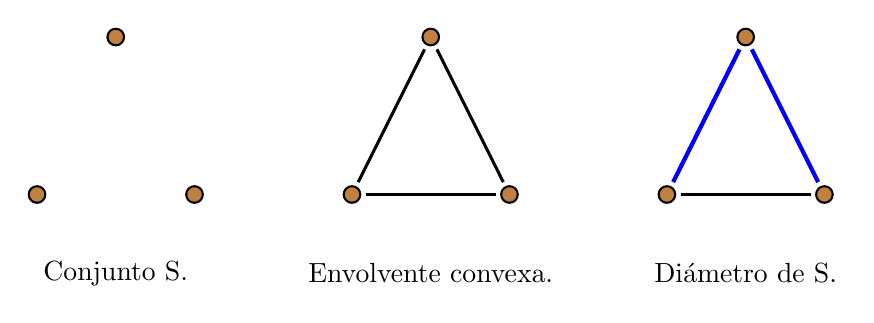
\begin{tikzpicture}
    %%%%%  Conjunto de puntos  %%%%%
    \node (0) [brownV]  at (1,1){};
    \node (1) [brownV]  at (0,-1){};
    \node (2) [brownV]  at (2,-1){};
    \node (T1)  at (1,-2) {Conjunto S.};

    %%%%% Envolvente convexa  %%%%%
    \begin{scope}[xshift=4cm]
      \node (3) [brownV]  at (1,1){};
      \node (4) [brownV]  at (0,-1){};
      \node (5) [brownV]  at (2,-1){};

      \draw [edge] (3) to (5);
      \draw [edge] (3) to (4);
      \draw [edge] (4) to (5);
      \node (T2)  at (1,-2) {Envolvente convexa.};
    \end{scope}

    %%%%% Componente debajo  %%%%%%
    \begin{scope}[xshift=8cm]
      \node (6) [brownV]  at (1,1){};
      \node (7) [brownV]  at (0,-1){};
      \node (8) [brownV]  at (2,-1){};

      \draw [blueE]  (6) to (7);
      \draw [blueE]  (6) to (8);
      \draw [edge]   (7) to (8);
      \node (T3)  at (1,-2) {Diámetro de S.};
    \end{scope}
  \end{tikzpicture}
\end{figure}
Como podemos notar, el diámetro contiene $3 > 2$ puntos.
\newline

Supongamos que cuando $|S| = k$, el diámetro de $S$ contiene dos puntos del polígono formado
por el cierre convexo de $S$.
\newline

¿Qué pasa cuándo nuestro conjunto de puntos $S$ aumenta en exactamente un punto? Existen 2 casos
interesantes para dar respuesta a esta pregunta, analicemos estos por separado
\begin{itemize}
\item Si el punto esta contenido\footnote{Casos: el punto esta al interior de $C(S)$, el punto esta en un segmento de $C(S)$.} en $C(S)$,
  terminamos. Pues, por hipótesis, nuestro diámetro ya contiene dos puntos en $C(S)$ y la anexión del punto distinguido [digamos $v$] modificaría
  al diámetro solo para aumentar $v$ (* esto lo podríamos  realizar tomando los puntos $x$ y $y$ más cercanos a $v$ que sean parte del diámetro, borar
  $xy$ de diámetro y añadir $xv$ y $vy$ a este).
  
\item Si el punto esta al exterior de $C(S)$, debemos calcular la envolvente convexa de $C(S')$, donde $S' = S + v$, esto lo podemos realizar
  econtrando las tangentes a $v$ con respecto de $C(S)$ y unirlas, este sería el nuevo cierre convexo. Lo anterior implica que $v$ será parte
  del polígono formado por la envolvente convexa (de otro modo, $v$ sería punto interno y se cubre en el caso anterior). Por ($*$) podemos anexar
  $v$ en $d$, y si el punto más cercano a $v$ es un extremo entonces basta con anexar ese segmento a $d$. Supongamos que cuando realizamos la
  unión de $v$ con $C(S)$ perdimos los puntos en $C(S)$ que también estaban en $d$ garantizados por la hipótesis, entonces ya tenemos a $v$ y como
  nadie en la envolvente pertenece a $d$, podemos anexar al vecino de $v$ en $C(S')$ a $d$ y terminamos.
\end{itemize}

\newpage
\textbf{3.} Dado un conjunto de puntos $S$ diseña un algoritmo que encuentre un polígono simple
cuyos vértices sean el conjunto $S$. \newline

\textbf{\textit{Solución.}} Para el diseño de este algoritmo tomaremos como base el algoritmo \code{Graham}
visto en clase, así, exhibamos el algoritmo
\begin{enumerate}
\item Primero debemos encontrar un punto distinguido $p_0$. Este punto puede ser cualquier punto y aquí nos podemos preguntar
  ¿Por qué cualquier punto? La respuesta es simple, todos los puntos serán parte de nuestro polígono y por tanto no da exactamente
  igual con cuál iniciar. Este paso tiene una complejidad contenida en $\mathcal{O}(1)$.
\item Ahora obtengamos un orden angular respecto a $p_0$, esto nos toma $\mathcal{O}(n \log_{2} n)$ por la cota de ordenamiento
  por comparaciones existente.
\item Ahora que ya tenemos un orden angular y un punto por el cuál iniciar, recorramos nuestros puntos tomando como siguiente, siempre,
  al próximo en el orden (así creamos una arista en cada iteración en el recorrido y lo guardamos, digamos en una lista) en sentido
  contrario a las manecillas del reloj\footnote{¿Esto necesario? No, es necesario ir en algún orden. No necesariamente este, sin embargo
  este orden es suficiente.}. Esto nos simplifica el detalle de conocer nuestras direcciones (validar) para poder regresar en caso de un
  giro en sentido contrario al requerido en \code{Graham}. Esto nos toma la cantidad de puntos en $S$, por tanto tenemos un orden
  $\mathcal{O}(n)$. Eventualmente llegaremos a $p_0$ y es en este momento que nuestro algoritmo termina regresando las aristas encontradas
  durante el recorrido.
\end{enumerate}

¿Por qué será cierto que nuestro algoritmo no encuentra aristas que se intersecten? Por el orden encontrado en ($2$).
\newline

\textit{Análisis de complejidad.} nuestro algoritmo tiene una complejidad en
\[\therefore \mathcal{O}(1) + \mathcal{O}(n \log_{2} n) + \mathcal{O}(n) \in \mathcal{O}(n \log_2 n).\]


\newpage
%%%%%%%%%%%%%%%%%%%% Problema02:
\textbf{4.} Un árbol de rango en un conjunto de $n$ puntos en el plano requiere
$\mathcal{O}(n \log n)$ de almacenamiento. Uno podría reducir los requisitos de
almacenamiento almacenando estructuras asociadas solo con un subconjunto de los
nodos en el árbol principal.

\begin{itemize}
\item Supongamos que sólo los nodos con profundidad $0, 2, 4, 6, \dotsm$ tienen
  una estructura asociada. Muestre cómo se puede adaptar el algoritmo de consulta
  para responder consultas correctamente.
\item Analice los requisitos de almacenamiento y el tiempo de consulta de dicha
  estructura de datos.
\end{itemize}

$\rhd$ \textbf{Solución:} Para este problema dividamos la solución en dos posibles
opciones:
\begin{enumerate}
\item ¿Cómo adaptamos nuestro árbol de rangos para que cumpla lo requerido en el primer
  punto? Como sabemos que un árbol, al menos, tendrá una raíz y las estructuras estarán
  ``colgadas'' de niveles pares. Entonces, la información respecto de $Y$ de los niveles
  impares estarán contenidas en el árbol colgado en su nivel par, inmediato, anterior.
  \newline
  
  Así, las consultas para los niveles pares se quedan exactamente iguales. Para los niveles
  impares consultamos respecto de $X$ y hacemos ``bracktraking'' al nivel par, inmediato,
  anterior para terminar la consulta en la estructura colgada en el nodo de ese nivel.
\item \textit{Análisis de almacenamiento.} El almacenamiento, aunque a primera vista se reduce
  en la cantidad de niveles pares, realmente las estructuras que estaban colgadas en estos niveles
  ahora formarán parte de las estructuras en niveles pares. El ahorro de almacenamiento es $\mathcal{O}(1)$,
  pues solo nos ahorramos las raíces de los niveles impares (que son, normalmente, hojas de los niveles
  pares).\newline
  
  \textit{Análisis de tiempo de consulta.} El tiempo de consulta para un elemento en un nivel par es el mismo,
  para un elemento en un nivel impar es el mismo en términos globales, pues el ``backtraking'' lo realizamos
  en tiempo $\mathcal{O}(1)$ y la consulta en la estructura ``colgada'' sigue siendo $\mathcal{O}(\log n) + k$.
  Como la consulta en árbol respecto a $X$ (árbol grande) es $\mathcal{O}(\log n)$, concluimos una
  complejidad de consulta en $\mathcal{O}(\log^2 n)$
\end{enumerate}
\textbf{Obs.} Para este problema estoy trabajando con un árbol de rango rectangulares.
\hfill $\lhd$

\end{document}
